\documentclass[11pt,letterpaper]{article}
\usepackage{authblk}
\usepackage{amsmath}
\usepackage{graphicx}
\usepackage{mathspec}
\setmainfont[BoldFont=Times_New_Roman_Bold.ttf,
             ItalicFont=Times_New_Roman_Italic.ttf, Mapping=tex-text]%
            {Times_New_Roman.ttf}
\setmathfont(Digits,Greek,Latin)%
            [ItalicFont=Times_New_Roman_Italic.ttf]%
            {Times_New_Roman.ttf}
\usepackage{microtype}
\usepackage{naaclhlt2016}
\usepackage{url}

% \naaclfinalcopy % Uncomment this line for the final submission
\def\naaclpaperid{***} %  Enter the naacl Paper ID here

% To expand the titlebox for more authors, uncomment
% below and set accordingly.
% \addtolength\titlebox{.5in}

\title{Target word prediction and paraphasia classification in spoken discourse}

% \author{Joel Adams \\ \textbf{Steven Bedrick} \\ \textbf{Jan Van Santen} \\
%         Center for Spoken Language Understanding \\
%         Oregon Health \& Science University \\
%         3181 SW Sam Jackson Pk Rd \\
%         Portland, OR USA 97239 \\
%         {\tt \{adamjo,bedricks,vansanten\}@ohsu.edu}
%       \And
%     Gerasimos Fergadiotis\\
%         Speech \& Hearing Sciences Department\\
%           Portland State University\\
%           PO Box 751\\
%           Portland, OR, USA 97207\\
%       {\tt gf3@pdx.edu}
%   \And
%   Kyle Gorman\\
%   Google, Inc.\\
%   79 9th Avenue \\
%   New York, NY 10011 \\
%   {\tt kbg@google.com}}

\author[1]{\textbf{Joel Adams}}
\author[1]{\textbf{Steven Bedrick}}
\author[2]{\textbf{Gerasimos Fergadiotis}}
\author[3]{\textbf{Kyle Gorman}}
\author[1]{\textbf{Jan van Santen}}
\affil[1]{Center for Spoken Language Understanding, Oregon Health \& Science University, Portland, OR}
\affil[2]{Speech \& Hearing Sciences Department, Portland State University, Portland, OR}
\affil[3]{Google, Inc., New York, NY}
\renewcommand\Authands{ and }

\date{}

\begin{document}

\maketitle

\begin{abstract}

We present a system for automatically detecting and classifying phonologically anomalous productions in the speech of individuals with aphasia.
Working from transcribed discourse samles, our system identifies neologisms, and uses a combination of string alignment and language models to produce a lattice of plausible words that the speaker may have intended to produce.
We then score this lattice according to various features, and attempt to determine whether the anomalous production represented a phonemic error or a genuine neologism.
This approach has the potential to be expanded to consider other types of paraphasic errors, and could be applied to a wide variety of screening and therapeutic applications.

\end{abstract}

\section{Introduction}

Aphasia is a neuropsychological condition in which an individual's ability to produce or comprehend language is compromised.
It can be caused by a number of different underlying pathologies, but can generally be traced back to physical damage to the individual's brain: tissue damage following ischemic or hemorrhagic stroke, lesions caused by a traumatic brain injury or infection, etc.
It can also be associated with various neurodegenerative diseases, as in the case of Primary Progressive Aphasia.
According to the National Institute of Neurological Disorders and Stroke, approximately 1,000,000 people in the United States suffer from aphasia, and aphasia is a common consequence of strokes (prevalence estimates for aphasia among stroke patients vary, but are typically in the neighborhood of 30\% \cite{Engelter:2006}).

\emph{Anomia} is a the inability to access and retrieve words during language production, and is a common manifestation of aphasia \cite{Goodglass:1997}.
An anomic individual will experience difficulty producing words and naming items, which can cause substantial difficulties in day-to-day communication.
Additionally, long-term communication difficulties associated with aphasia in general have been shown to affect the psychological well-being of people with aphasia as well as their families \cite{Kristensson:2015,Gaete:2008,vanDijk:2015}.

The process of screening for, diagnosing, and assessing anomia is typically manual in nature, and requires substantial time, labor, and expertise.
Compared to other neuropsychological assessment instruments, aphasia-related assessments are particularly difficult to computerize, as they typically depend on subtle and complex linguistic judgments about the phonological and semantic similarity of words, and also require the examiner to interpret phonologically disordered speech.
Furthermore, the most commonly used assessments focus for practical reasons on relatively constrained tasks such as picture naming, which may lack ecological validity \cite{Mayer:2003}.

In this work, we describe an approach to automatically detecting and analyzing certain categories of word production errors characteristic of anomia in connected speech.
Our approach is a first step towards an automated anomia assessment tool that could be used cost effectively in both clinical and research settings,\footnote{As in the computer-administered (but manually-scored) assessments developed by Fergadiotis and colleagues \cite{Fergadiotis:2015,Hula:2015}. } and could also be applied to other disorders of speech production.
The method we propose uses statistical language models to identify possible errors, and employs a phonologically-informed edit distance model to determine phonological similarity between the subject's utterance and a set of plausible ``intended words.''
We then apply machine learning techniques to determine which of several categories a given erroneous production may fall into.
We show XXXX % TODO: what do we show?

\subsection{Anomia and Paraphasias} % (fold)
\label{sub:anomia_and_paraphasias}

% subsection anomia_and_paraphasias (end)

Anomia can take several different forms, but in this work we are concerned with \emph{paraphasias},
which are unintended errors in word production.\footnote{Note that individuals \emph{without} any sort of language disorder do occasionally produce errors in their speech; this fact has led to a truly shocking amount of study by linguists.
Frisch \& Wright \shortcite{Frisch:2002} provide a reasonable overview of the background and phonology of the phenomenon.} % TODO: Kyle, Gerasimos, do either you have a better refrence for this?
There are several categories of paraphasic error. \emph{Semantic errors} arise when an individual unintentionally produces a semantically-related word to their original, intended word (their ``target word'').
A classic semantic error would be saying ``cat'' when one intended to say ``dog.''

\emph{Phonemic} (sometimes called ``formal'') errors occur when the speaker produces an unrelated word that is \emph{phonemically related} to their target: ``mat'' for ``cat'', for example.
It is also possible for an erroneous production to be \emph{mixed}, that is both semantically and phonemically related to the target word: ``rat'' for ``cat.''
Individuals with anomia also produce \emph{unrelated} errors, which are words that are neither semantically or phonemically related to their intended target word: for example, producing ``skis'' instead of ``zipper.''

Each of these categories shares the commonality that the word produced by the individual is a ``real'' word. There is another family of anomic errors, \emph{neologisms}, in which the individual produces \emph{non-word} productions.
A neologistic production may be phonemically related to the target, but containing phonological errors: ``[dɑɪnoʊsɔɹ]'' for ``dinosaur.''
These are often referred t as \emph{phonological} paraphasias.
Alternatively, the individual may produce \emph{abstruse neologisms}, in which the produced phonemes bear no discernable similarity to any ``real'' lexical item (``[æpməl]'' for ``comb''\footnote{This example was taken from a corpus of responses to a confrontation naming test \cite{Mirman:2010}, in which the subject is shown a picture and required to name its contents. As such, in the case of this specific error, we have \emph{a priori} knowledge of what the target word ``should'' have been. Obviously, in a more naturalistic task or setting, we would not have this advantage.}).

A full discussion of the theoretical basis for this typology of paraphasias is beyond the scope of this paper.
That said, it is worth nothing that the standard model explaining these sorts of anomic errors is Dell's two-step word production model \cite{Dell:1997,Dell:1986}.
In Dell's model, language production occurs in two primary phases.
First, the speaker forms some semantic representation of what they wish to say, and accesses the lemma form of that word.
Then, those selected lexical items are translated into spoken language.

Under this model, then, there are two primary ways that paraphasic productions can occur: the ``wrong'' lexical item may be selected (as in the case of a semantic error or an unrelated error), and/or the translation process from lexical item to produced speech may go awry, resulting in formal (or other such phonemic) errors.
When problems occur in both steps of the process, we see a mixed error (i.e., an error containing both phonological and semantic components).

The present work focuses exclusively on neologisms, both of the phonological variety as well as the abstruse variety. However, our fundamental approach can be extended to include other forms, as described in section~\ref{sub:future_work}.

Typical methods of diagnosing, staging, and otherwise characterizing anomia involve determining the number and kinds of paraphasias produced by an individual while undergoing some structured language elicitation process, for example a confrontation naming test (see \cite{Kendall:2013} and \cite{Brookshire:2014} for examples of such a study).
As alluded to previously, producing these counts and classifications is a complex and laborious process.
Furthermore, it is also often an inherently subjective process: are ``carrot'' and ``banana'' semantically related?
What about ``hose'' and ``rope''?

Reliability estimates of expert human performance at paraphasia classification in confrontation naming scenarios reflect the difficulty in this task. One recent study reported a kappa-equivalent score of 0.76 --- a score that that is certainly acceptable, but that leaves much room for disagreement on the status of specific erroneous productions \cite{Minkina:2015}.
Other reported scores fall in a similar range \cite{Kristensson:2015}, including when the productions are from neurotypical individuals \cite{Nicholas:1989}.
Automating this aspect of the task would not only improve efficiency, but would also decrease scoring variability.

Having a reliable, automated method to analyze paraphasic errors would also expand the scope of what is currently possible in terms of assessment methodologies.
Confrontation naming tests are often used (both in the clinic as well as in research settings) not because they are thought to optimally characterize the speech capabilities of their subjects, but rather out of concerns regarding feasibility of scoring.
Naturalistic language samples may be more ecologically valid, but such data present a very complex and challenging scoring scenario (for example, see \cite{Nicholas:1993,Berndt:2000,Rochon:2000}), and so practitioners often eschew them in favor of simpler, more structured assessments.

Notably, the approach we outline in this paper is explicitly designed to work on samples of natural, connected speech---though it did grow out of work that the authors are currently doing on automated confrontation naming test scoring.
It is our hope that, by enabling automated calculation of  error frequencies and types on narrative speech, we might make using such material far easier in practice than it is today.

\section{Methods}

Our overall approach was as follows.
Beginning with transcribed narrative samples from people with aphasia, we used a corpus-driven method to identify possible neologisms in the subjects' speech.
Once we have identified candidate neologisms, we must
Next, for each neologism, we used an n-gram language model to build a weighted lattice of plausible ``target words'' (see figure~\ref{fig:sample_lattice} for an unweighted example of such a lattice).
For each sentence, we then compute a metric of phonological similarity between the erroneous utterance produced by the subject and the candidate target words.
We then attempt to classify this production as either a phonological paraphasia or an abstruse neologism.
We will describe each step of the process in detail below, beginning with our the data set.

\subsection{Dataset} % (fold)
\label{sub:dataset}

For the work described in this paper, we relied on the AphasiaBank project \cite{MacWhinney:2011}, which has assembled a large database of transcribed interactions between examiners and people with aphasia, nearly all of whom have suffered a stroke.
Notably, AphasiaBank also includes some number of transcribed sessions with neurotypical controls.
Each interaction follows a common protocol and script, and is transcribed in great detail using a standardized set of annotation guidelines.
The transcripts include word-level error codes, according to a spectacularly detailed taxonomy of errors and associated annotations.
Erroneous productions are not simply flagged as erroneous.
In the case of semantic, formal, and phonemic errors, the word-level annotations include a ``best guess'' on the part of the transcriber as to what the speaker's intended production may have been.
In the case of non-lexical productions (phonemic errors, neologisms, etc.), the annotations include an IPA transcription of the subject's precise utterance.
In some cases, the transcribers include information about gestures and other non-verbal communication that the subjects may have produced.
The transcripts are stored in the CLAN (Computerized Language Analysis) format \cite{MacWhinney:2000}, and are therefore highly amenable to automated analysis.

% TODO(Joel): I was surprised to see you say that CLAN was "highly amenable", as it alwas seemed to me like a total mess without much of a clear schema. I know CHILDES is available as schematic XML...is that also true for AphasiaBank? If so, I'd say it's worth a small amount of time to chuck the CLAN annotations (and whatever you're using to deal with them) and replace them with a bit of XML handling. --KBG.
% SDB sez: "highly amenable" was me being generous and charitable. "Total mess without clear schema" is far more accurate. AphasiaBank is *not* available as schematic XML, but the first thing I had Joel do upon starting this project was to come up with a lightweight XML schema and transform the CLAN files into XML. It was a god-send.
% SDB also sez: Seriously, the developers of CLAN ought to be ashamed of themselves for foisting their bizarre HCI ideas upon poor, non-technical linguists who don't know any better. It's like some sort of unholy vi-emacs hybrid- all the inscrutable command modes of vi, with the baroque multi-stage keyboard inputs of emacs.

Each transcribed session consists of a prescribed sequence of language elicitation activities, including a set of personal narratives (e.g., ``Tell me a story about an important event that happened to you'', ``Do you remember when you had your stroke? Please tell me about it.''), standardized picture description tasks, a story retelling task (involving the story of \emph{Cinderella}), and a procedural discourse task (in which the subjects are asked to describe for the examiner the process of making a peanut-butter and jelly sandwich).

In addition to the narrative sessions, each subject's data also includes the results of a battery of standardized assessments, including a confrontation naming test, the Aphasia Quotient sub-test of the Western Aphasia Battery, and so forth.

We obtained an up-to-date copy of the AphasiaBank database, and applied a series of minor normalizations as a first step in our analytical pipeline. First, we harmonized the names by which examiners referred to the various tasks, as this varied slightly from study site to study site (e.g., one site referred to the ``Important event'' task, while another referred to ``Important\_Event''), and dealt with several other such minor orthographic irregularities across study sites.

Less trivially, we collapsed certain word-level error codes.
As an example, the AphasiaBank protocol includes a special annotation used to indicate that a given neologism error represents an utterance that recurs frequently within a particular subject, as occasionally happens with individuals with aphasia (e.g., an individual might repeatedly utter the phonemes XXX). % TODO: From Joel, get example phonemes!
Since the present analysis was not concerned with this aspect of the transcripts, we collapsed instances of this and several other similarly specific error codes into their more general forms.

Certain non-standard productions that are nevertheless typical of a dialect (``gotta'', etc.) are occasionally labeled by the AphasiaBank transcribers as such, along with their ``canonical'' form (e.g. ``got to'' for ``gotta''). In these cases, we replaced the ``true'' production with its canonical form. This was motivated by the fact that we would be using  language models that were not explicitly trained on conversational speech, and we did not want incidental dialect usage of this sort to complicate matters.

Finally, we transformed the human-generated IPA representation of non-word productions into a relatively impoverished graphemic representation (using the inverse of the process described in section~\ref{sub:phonological_similarity}).
Our purpose in doing this was to simulate a scenario where we did \emph{not} have high-quality human-produced phonetic transcriptions. Obviously, one major obstacle to using narrative samples in any sort of clinical assessment is the need for transcription.
Two of the most plausible solutions to this problem are automatic speech recognition (ASR)\footnote{See Fraser et al. \shortcite{Fraser:2015} for a detailed discussion of the implications of using ASR on the speech of individuals with aphasia} and/or the use of \emph{non-expert} transcribers to produce ``quick-and-dirty'' transcripts (perhaps via Amazon Mechanical Turk, or some other such crowd-sourced platform).

In the case of ASR-derived transcripts, we would presumably have access to some sort of phonetic representation of what was said by the subject, though this representation would almost certainly be incomplete and error-prone (ASR systems are particularly bad at handling non-word productions of any sort).
Even in the less-challenging case of transcripts produced by non-expert humans, we would of course not find the professional-quality IPA transcriptions found in the AphasiaBank database.
We would instead be working with a ``best effort'' attempt at rendering what the transcriber heard the subject produce.

We therefore anticipate that in any sort of ``real-world'' scenario of use, our system will need to operate with imperfect phonetic information.
As such, for this study, we modified the phonetic transcripts found in the AphasiaBank data to something approximating ``standard'' English orthography.

We next chose two of the AphasiaBank personal narrative tasks--- describing the individual's stroke, and telling the story of an important event that happened sometime during the individual's life--- to work with, and excerpted the intervals containing those sections from each transcript.
This resulted in XXX sentences from YYY individuals. % TODO: Joel, numbers?
We then identified sentences containing instances of our errors of interest: phonological paraphasia (AphasiaBank codes ``p:n'', ``p:m'', and ``n:k'') or abstruse neologism (``n:uk'').
Note that the distribution of errors within sentences was relatively Zipfian, in that the majority of error-containing sentences contained a single error, followed somewhat distantly by sentences containing two errors, with a relatively steep dropoff thereafter.
For the present study, we restricted our analysis to sentences that contained either one or two errors.

Our reasoning for this restriction was that we do not presently have a theoretically-informed model of what, if any, relationship there may be between multiple errors within a sentence. 
However, it seems quite likely that the errors occurring in a sentence containing (for instance) five paraphasic errors might be somehow related to one another.
We anticipate exploring this phenomenon in the future (see section~\ref{sub:future_work}).

Our final data set consisted of XXX sentences from YYY individuals, containing errors from ZZZ distinct categories. % TODO: Joel, numbers

% subsection dataset (end)

\subsection{Identification of Neologisms} % (fold)
\label{sub:identification_of_neologisms}

We next turned to the question of identifying neologisms in our sentences.
Simply using a standard dictionary to determine lexicality could result in numerous ``false positives,'' driven largely by proper names of people, brands, etc.
To avoid this, we used the SUBTLEX-US corpus \cite{Brysbaert:2009} to identify neologisms. SUBTLEX-US was build using subtitles from English-language television shows and movies, and Brysbaert and New have demonstrated that it correlates with a number of psycholinguistic behavior measures (most notably, naming latencies) better than better-known frequency norms such as those derived from the Brown corpus or CELEX-2.

Note that, in the present analysis, this step in our pipeline was something of a contrived exercise, as (thanks to the detailed annotations present in the AphasiaBank transcripts) we already ``knew'' which tokens represented neologisms.
However, in a ``real-world'' scenario, when we did \emph{not} know \emph{a priori} which tokens represented non-word productions, this step would be of particular importance, and we wished to simulate it with as much fidelity as possible.
Furthermore, recall that while the present analysis only concerns itself with non-word productions, there are a number of paraphasia types in which a valid word is produced.
Determining which productions represent a semantic or formal error is much more complex than simply performing a corpus lookup.
We expect this stage of our pipeline to grow in complexity in the future.

Upon identifying a possible non-word production, recall that our next goal is to determine whether it represents a \emph{phonemic} error (substituting ``[dɑɪnoʊsɔɹ]'' for ``dinosaur'') or an \emph{abstruse neologism} (a completely novel sequence of phonemes that does not correspond to an actual word).
To help accomplish this, we use a language model to identify plausible words that \emph{could} fit in the slot occupied by the erroneous production, and produce a lattice of these candidate target words (i.e., words that the subject may have been intending to produce, given what we know about the context in which they were speaking).

% subsection identification_of_neologisms (end)

\subsection{Language Model Construction} % (fold)
\label{sub:language_model_construction}

Our language models for this study were built using the New York Times section of the Gigaword newswire corpus \cite{Gigaword}. 
We tokenized using the standard Penn Treebank tokenizer, left stopwords intact, and case-folded all sentences to upper-case.
Cardinal numbers were collapsed into a category token, as were ordinal numbers and dates (each category was given its own token).
We used the the OpenGrm-NGram language modeling toolkit \cite{Roark:2012} to build the language models themselves, using an n-gram order of 4, with Kneser-Ney smoothing \cite{Kneser:1995ib}. 

We investigated two different language model approaches.
In the first approach, we trained our models on the totality of the New York Times data.
However, given that many of the AphasiaBank narrative tasks consist of fairly topic-constrained language (e.g., the Cinderella retelling, the personal narrative about the subject's stroke, etc.), we hypothesized that we would get better results (i.e., higher-quality word predictions) if we could train our models on a more focused set of data.

To accomplish this, we used the Gensim topic modeling package \cite{Rehurek:2010} to train a Latent Dirichlet Allocation topic model \cite{Blei:2003} on the entire New York Times data set.
For the present analysis, we instructed the model to use 20 topics.
We next projected the text of each of the narrative samples into the topic space described by the model, and calculated the centroids for each of the narrative task.
This gave us, for example, the estimated topic distribution most representative of the Cinderella retellings, the PB\&J instructions, and so on.

Then, we calculated the Euclidean distance between each article in the New York Times corpus and each narrative task's centroid.
This allowed us to determine the ``most similar'' New York Times articles for each narrative task, which in turn enabled us to produce ``task-specific'' subsets of the larger corpus.

The end result was that we were able to produce a more topically homogeneous collection of New York Times articles to use in training per-narrative-task language models.
We ended up identifying two of the narrative tasks--- ``tell me about your stroke'' and ``tell me about an important event''--- as fitting particularly well into the topic space described by the New York Times data, and focused on those two tasks for the remainder of the analysis.

% Joel will give me example words from the two tasks's centroids, and also some info about a) exactly how many NYT articles we used for both, and b) some of the most representative article titles

In this study, we evaluated the performance implications of using either the omnibus model or a task-specific model.
In future work (see section~\ref{sub:future_work}), we anticipate experimentation with interpolating between the two.

\subsection{Lattice Construction \& Scoring} % (fold)
\label{sub:lattice_construction_scoring}

We next produced lattices representing the set of possible sentences that the subject could plausibly have been intending to produce. 
We did this by constructing a finite-state acceptor whose arcs represent words in the sentence.
At the point in the produced sentence where our error detection system indicated that a non-word production occurred, we represent the anomaly by the union of all possible words in our lexicon (see figure~\ref{fig:sample_lattice} for an example sentence lattice). 

We next computed weights for the sentence lattice by composing it with our language model.
Then, we pruned our lattice by computing the $n$-best paths through the resulting weighted automaton in the Tropical semiring (for this analysis, $n$ was 1,000). 
Finally, we scored each possible remaining candidate production with the final forward probability of the version of the sentence containing that candidate.

\begin{figure}[t]
\centering
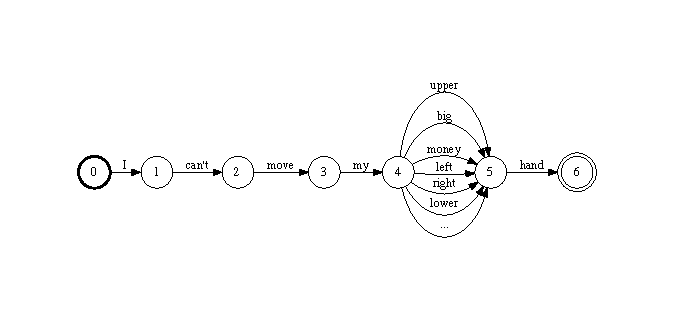
\includegraphics[width=3.5in]{lattice.pdf}
\label{fig:sample_lattice}
\caption{An example candidate word lattice for the production ``I can't move my [vɑɪ] hand.''}
\end{figure}

% subsection lattice_construction_scoring (end)

\subsection{Phonological Similarity} % (fold)
\label{sub:phonological_similarity}

At this point in the process, we have the following information about each erroneous production: a best-guess orthographic transcription of what the individual actually produced, and a ranked list of plausible lexical that they could potentially have been attempting to produce, together with probability estimates for each production.
Recall that our goal is to determine whether the erroneous production was a phonemic paraphasia or an abstruse neologism.
In order to make this determination, we must know whether the subject's utterance is phonemically related to any of the plausible target words.

Determining phonemic similarity can be done in a number of ways. 
In this work, we compute several different metrics of phonological similarity, and then use the resulting scores as inputs to a classifier. 
These methods fall into two general categories: rule-based and statistical.

Many aphasia assessment instruments include strict rule-based guidelines on how to determine phonological similarity.
For example, the scoring instructions for the Philadelphia Naming Test (PNT) include detailed rules that take into account the number of shared phonemes and syllables that two productions may have in common \cite{Roach:1996sp}.
The annotation standards used by the AphasiaBank project also include an algorithm for determining if two words are phonologically related or not.
As an example of one of the AphasiaBank rules, monosyllabic productions with an onset, vowel nucleus, and coda must match two of the three elements of a target word in order to be considered phonologically similar \cite{MacWhinney:2000}.
Both the PNT and the AphasiaBank rule sets are designed to optimize for coding consistency and ease of use on the part of linguistically informed human annotators.

As described in section~\ref{sub:related_work}, besides rule-based phonological similarity metrics, there exist variety of statistical approaches for determining phonological similarity. 
In this work, we employ an edit-distance based metric that uses phoneme category rules, and assigns smaller substitution costs to replacement of ``similar'' phonemes (i.e., a substituting one unvoiced fricative for another unvoiced fricative will cost less than substituting an unvoiced fricative for a voiced stop).

We first convert our best-guess orthographic representation of the subject's non-lexical production to an estimated phonological representation using the Phonetisaurus grapheme-to-phoneme toolkit \cite{Novak:2012}. 
Next, we compute the phonologically-aware edit distance for each (production,candidate target) pair, and also apply the Philadelphia Naming Test phonological similarity rules. We use the CMU Pronouncing dictionary to obtain phonetic representations of the candidate target words.

At this point, we now have, for each error, a ranked list of plausible candidate target words, along with probability and phonological similarity scores for each candidate. We are now ready to attempt to classify the errors.

% subsection phonological_similarity (end)

\subsection{Classification, Re-ranking, \& Evaluation} % (fold)
\label{sub:ranking_scoring}

To determine the category of our error productions--- again, between productions representing phonological errors such as ``[dɑɪnoʊsɔɹ]'' for ``dinosaur'', and productions representing abstruse neologisms--- we trained a binary classifier using features representing the characteristics of the candidate target word space surrounding the erroneous production.
Our intuition was that phonemic errors were much more likely than abstruse neologisms to have highly-ranked candidate target words that were also phonologically similar to the subject's actual production. % TODO: Kyle, Joel: does this sentence make any sense at all?

We used the Scikit-learn Python machine learning library \cite{scikit-learn} to train a Support Vector Machine classifier,\footnote{Our choice of classifier was driven largely by a desire for simplicity and a need for a classifier that could easily accomodate both continuous and categorical features.} and our features were a concatenated vector of, for each of the $n$-best candidate target words: 

\begin{enumerate}
    \item The forward probability of the candidate (normalized across the $n$-best candidates);
    \item The candidate's phonological similarity to the production, according to the AphasiaBank guidelines
    \item The candidate's phonological similarity to the production, according to the PNT guidelines % TODO: Joel, are we actually using this, or did we decide to ditch it?
    \item The candidate's phonologically-informed edit distance from the production
\end{enumerate}

We performed leave-one-out cross-validation of our classifier across 

% subsection ranking_scoring (end)

\section{Results} % (fold)
\label{sec:results}

% (end)

\section{Related Work \& Discussion} % (fold)
\label{sec:discussion}

While our results were 

\subsection{Related work} % (fold)
\label{sub:related_work}

As far back as Shannon's word-guessing game \cite{Shannon:1951}, researchers have sought to leverage the statistical regularities in natural language to predict missing or subsequent words. 
In practice, however, this proves to be a surprisingly challenging problem.
Language occurs at levels beyond simply choosing lexical items, and local statistical characteristics of language often fail to capture syntactic and semantic patterns. 
Zweig \& Burges \shortcite{zweig-burges:2012:WLM} provide an enlightening discussion on the limitations of relying on n-gram guessing for syntactically complex tasks such as ``identify the missing word in the sentence,'' and also describe a very challenging language model evaluation task built around this problem.
They tested a variety of language modeling approaches using their task, and report that well-trained generative n-gram models achieve correct predictions $\approx 30\%$ of the time,\footnote{A finding that we can corroborate with the results presented in this paper.} while approaches using Latent Semantic Analysis\cite{Deerwester:1990vi} can achieve scores in the mid-40s. 
State-of-the-art performance on the their word prediction task typically use recurrent neural network langage models,\footnote{See De Mulder et al. \shortcite{DeMulder:2015dy} for a recent review on this subject.} and the best scores are in the mid-$50\%$ range \cite{mirowski-vlachos:2015:ACL-IJCNLP,NIPS2013_5165}. 

In our case, the nature of our data renders this task even more challenging. Our sentences are often short and agrammatical (often missing or mis-using determiners, for example), and are produced by individuals with impaired language ability. 



Using phonemic similarity to identify potential lexical items: \cite{Han:2011,Choudhury:2007}
    - much related work in the text normalization literature \cite{Sproat:2001}


Computational analysis of aphasic speech: tends to either involve computational analysis of carefully annotated data, or looks at higher-level syntactic features rather than low-level lexical analysis as in our work.
    Using aphasiabank \cite{MacWhinney:2011}
    automatic sub-typing from narrative transcripts\cite{Fraser:2014bg}
    statistical parsing to detect\cite{fraser-EtAl:2014:W14-34}
        Syntactic analysis of same: \cite{Goodglass:1994}
Segmentation of aphasic speech: \cite{Fraser:2015}


% subsection related_work (end)


% (end)

\section{Conclusion \& Future Work} % (fold)
\label{sec:conclusions}

Limitations:
    - We are only using sentences with 1 error- excluding sentences with >1 error (N = 1,866)
    - more generally, we don't have a clean idea of how/whether sentences with multiple errors are different from mono-error sentences
        - open question for future work: are paraphasic errors within a sentence related to one another in some way?
        - our general finite-state approach can be generalized to sentences with additional errors, and we will explore such possibilities in future work!

\subsection{Future Work} % (fold)
\label{sub:future_work}

Future work:
    - better LM, better phonology, etc. etc.
        - interpolation between omnibus and task-specific LMs
        - using backward probability as well as forward probability
    - using PoS/syntax to help word prediction
    - subject-level adaptation: using characteristics of the subject and their language to help identify erroneous productions
    - use of surprisal


% subsection future_work (end)

% section: conclusion (end)

\section*{Acknowledgments}

This material is based upon work supported in part by the National Institute on Deafness and Other Communication Disorders of the National Institutes of Health under awards R01DC012033 and R03DC014556.
The content is solely the responsibility of the authors and does not necessarily represent the official views of the granting agencies or any other individual.


\bibliography{target_word_prediction,other_refs,kbg_refs}
\bibliographystyle{naaclhlt2016}

\end{document}
